%!TEX root = paper.tex
\section{Plant Seedlings Classification}
\subsection{Data}

\indent{\indent The dataset is a part of the database have been recorded at Aarhus University Flakkebjerg Research station in a collaboration between University of Southern Denmark and Aarhus University. Images are avaliable to researches at \url{https://vision.eng.au.dk/plant-seedlings-dataset/}. The specific of the dataset is that recorded plants are in different growth stages since detecting weed in it's early stage is the thing makes the task problematic. }

\indent{The dataset contains 960 unique plant images of 12 species. The sizes of plant classes are not balanced among themselves - they range from 221 to 654 labeled samples for each class. Original images are cropped by plant boundaries, but their resolutions varyes from 50x50px to 2000x2000px. Also, images have a different background - some of them on the ground, other on the marked paper.}
\begin{figure}[h]
    \centering
    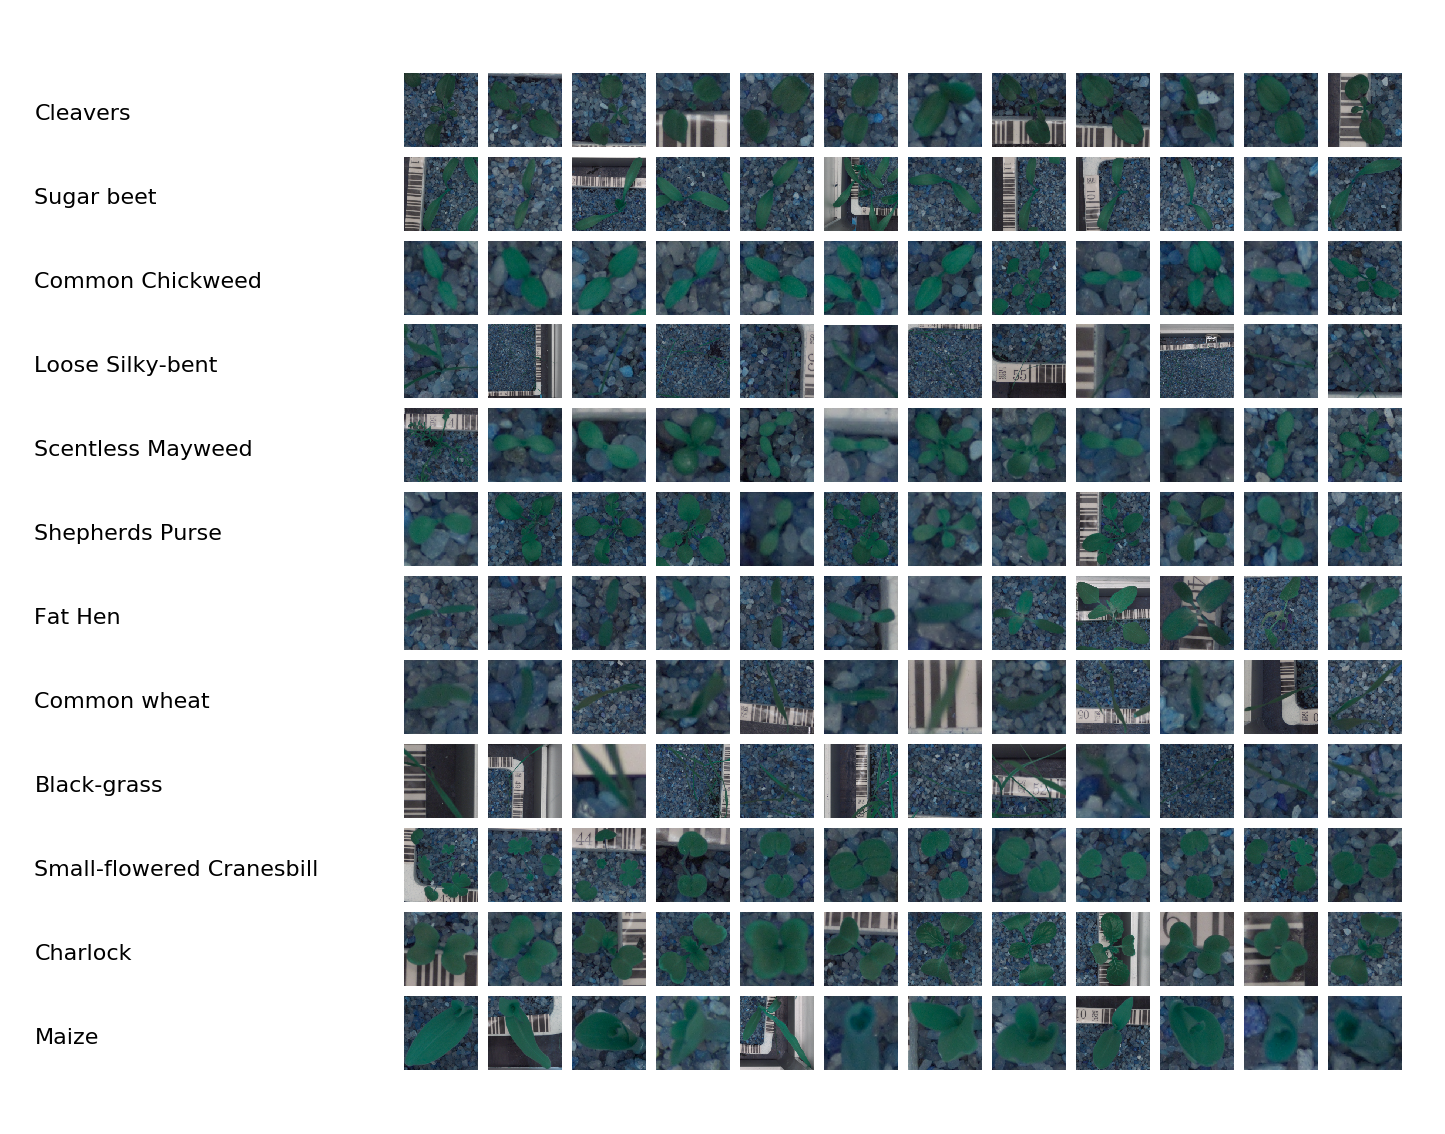
\includegraphics[height=7.5cm, width=10cm]{first_view_grid_1}
    \caption{Data overview}
    \label{fig:1}
\end{figure}

\subsection{Data preprocessing}
\indent{\indent We have three stages of data preprocessing.}

\indent{Firstly, we reduce resolution of all images to the same resolution 200x200px using bilinear interpolation. The main idea of bilinear interpolation that the new image pixel is the weighted sum of neighboring pixels of the original image. It helps to decrease computational complexity and build normalized features.}

\indent{Secondly, the objects of our study are plants and they are painted green. Therefore, we can create a mask that filters the range of green channel and ignores the other pixels. For these purposes the HSV (Hue Saturation Value) color model is suitable representation. In the BGR format, the value of each component depends on the amount of light hitting the object. HSV allows us to distinguish between image color and brightness. Hue, saturation and value let us set the lower and upper borders of the shades of a certain color, in this case –– green. Then we merely mark the pixels in the green range and get a color mask (Fig. \ref{fig_f_ seg_step_2}). Now we apply the operation of logical multiplication to the original image, assign the value of the background pixels to a black value and get a segmented plant.}

\threeimage{seg_step_1}{seg_step_2}{seg_step_3}{Source image}{Mask}{Segmented image}

\indent{Thirdly, }

\subsection{Feature selection?}

\indent{\indent Features of the images define their content. We recognise the information images provide us with taking into account a great number of features. Then we answer what do we see exactly. The same process can be projected on image classification task: image features let the classifier propose the output decision. Another advantage of the approach is that it reduces feature space for a machine learning algorithm. We often need only a part of the information image is carrying, hence we don't need to process and interpret all the pixels, what can lead to extra computational expences.}

\indent{ Selecting features is a complicated and convoluted research area itself, the assertion if supported by the variety of feature types and the need of presenting essential properties on the equal basis with the previous assertion.}

\indent{ As dicucussed before, we need to define the set of features describing the dataset in the best way. Supposed features must meet the following criterion:}

\begin{itemize}
    \item The feature space should be low-dimensional
    \item The features should not be correlated or be correlated as less as possible
    \item Selected features should represent the content of an image as fully as possible
\end{itemize}

\indent{ We are going to group selected features and define them.}

\subsection{Color features}

\indent{\indent Overviewing the dataset we can notice that all the plant species are mostly green. Additionally, images were recorded under specific conditions. We will use RGB color model, which stands for red, green and blue colors, and calculate features described below.}

\begin{figure}[h]
    \centering
    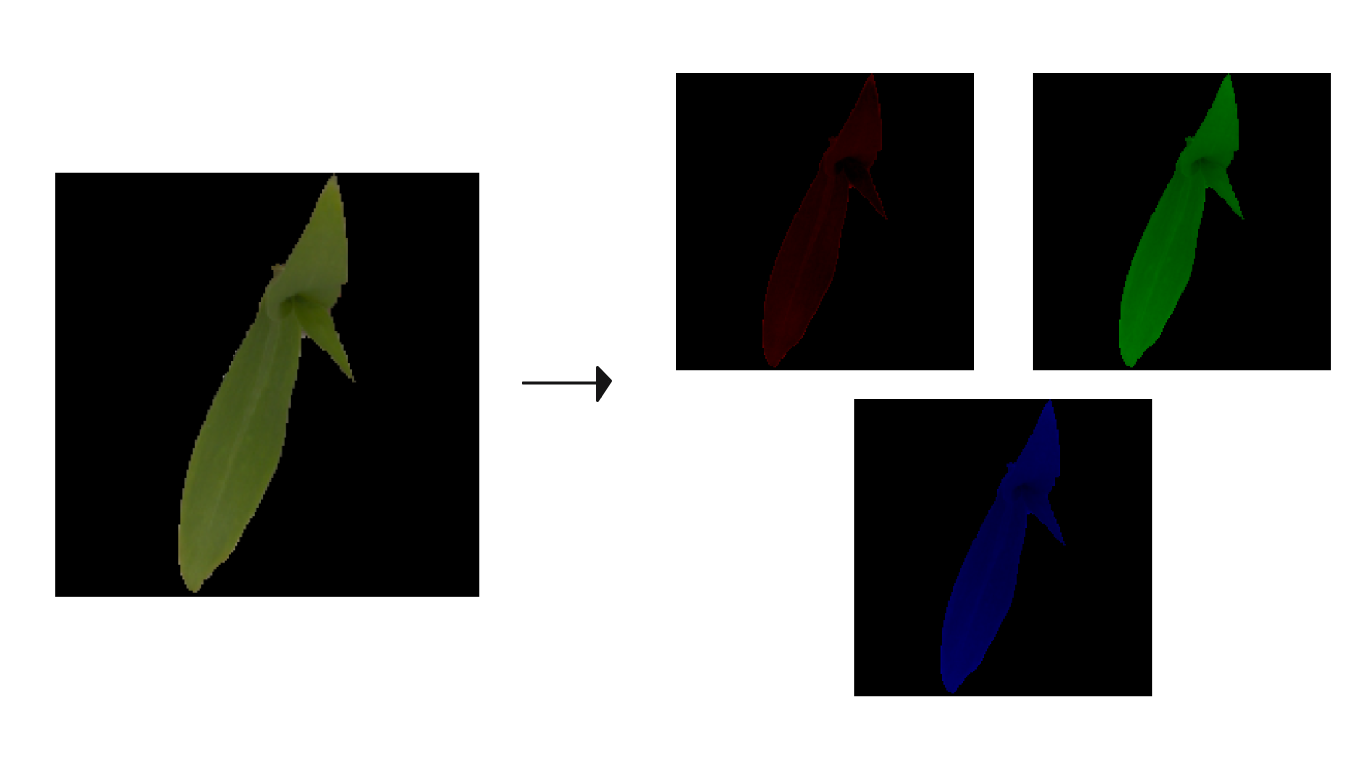
\includegraphics[height=5.5cm, width=10cm]{to_rgb_sample_1}
    \caption{RGB transformation}
    \label{fig:2}
\end{figure}

\vspace{3cm}
\indent{Let $\{x^{(k)}\}_{i=1}^N$, where $k = 1, 2, 3 $ –– an index of a channel in RGB color space respectively, $N$ –– total number of the image pixels, $x^{(k)}_i$ –– $i$-th pixel of the $k$-th channel. We will compute sample mean and standard deviation for each channel:}

\begin{equation}
	\label{eq:1}
	\overline{x^{(k)}} = \frac{1}{N}\sum_{i=1}^{N}x^{(k)}_i 
\end{equation}

\begin{equation}
	\label{eq:2}
	 s^{(k)} = \sqrt{\frac{1}{N}\sum_{i=1}^{N}(x^{(k)}_i - \overline{x^{(k)}})^2} 
\end{equation}

\subsection{Shape features}

\indent{\indent \textbf{Total perimeter}}

\indent{In this feature we will count the sum of perimeters of all the areas bounded by contours:}

\begin{equation}
	\label{eq:3}
	 P = \sum_{i=1}^{K}p_i,
\end{equation}
where $p_i$ –– $i$-th perimeter, $K$ –– number detected bounding contours

\textbf{Total area}

\indent{It includes all the areas bounded by contours:}

\textbf{Maximal contour area}

\textbf{Number of bounding contours}

\indent{Segmentation output may result in image divided in separate parts of the plant. We decided to use it and compute the number of bounding contours. We will use the boundary tracing algorithm for the boundary extraction. The designated algorithm \cite{cv1985contours} was implemented in OpenCV \cite{opencv2000python} library for the Python programming language.}

\textbf{Rectangularity}

\textbf{Circularity}


\subsection{Classification}
